%%% Version 3.3 Generated 2016/11/10 %%%
%%% You will need to have the following packages installed: datetime, fmtcount, etoolbox, fcprefix, which are normally inlcuded in WinEdt. %%%
%%% In http://www.ctan.org/ you can find the packages and how to install them, if necessary. %%%
%%%  NB logo1.jpg is required in the path in order to correctly compile front page header %%%

\documentclass[utf8]{frontiersSCNS} % for Science, Engineering and Humanities and Social Sciences articles
%\documentclass[utf8]{frontiersHLTH} % for Health articles
%\documentclass[utf8]{frontiersFPHY} % for Physics and Applied Mathematics and Statistics articles

%\setcitestyle{square} % for Physics and Applied Mathematics and Statistics articles
\usepackage{url,hyperref,lineno,microtype,subcaption}
\usepackage[onehalfspacing]{setspace}
\usepackage{color, soul}
\usepackage{amsmath}
\usepackage{booktabs}
\usepackage{multirow}

\linenumbers


% Leave a blank line between paragraphs instead of using \\


\def\keyFont{\fontsize{8}{11}\helveticabold }
\def\firstAuthorLast{Sample {et~al.}} %use et al only if is more than 1 author
\def\Authors{First Author\,$^{1,*}$, Co-Author\,$^{2}$ and Co-Author\,$^{1,2}$}
% Affiliations should be keyed to the author's name with superscript numbers and be listed as follows: Laboratory, Institute, Department, Organization, City, State abbreviation (USA, Canada, Australia), and Country (without detailed address information such as city zip codes or street names).
% If one of the authors has a change of address, list the new address below the correspondence details using a superscript symbol and use the same symbol to indicate the author in the author list.
\def\Address{$^{1}$Laboratory X, Institute X, Department X, Organization X, City X , State XX (only USA, Canada and Australia), Country X \\
$^{2}$Laboratory X, Institute X, Department X, Organization X, City X , State XX (only USA, Canada and Australia), Country X  }
% The Corresponding Author should be marked with an asterisk
% Provide the exact contact address (this time including street name and city zip code) and email of the corresponding author
\def\corrAuthor{Corresponding Author} 

\def\corrEmail{email@uni.edu}




\begin{document}
\onecolumn
\firstpage{1}

\title[Running Title]{Predicting age with machine learning, using synchronized speech and MEG recordings in children} 

\author[\firstAuthorLast ]{\Authors} %This field will be automatically populated
\address{} %This field will be automatically populated
\correspondance{} %This field will be automatically populated
 
\extraAuth{}% If there are more than 1 corresponding author, comment this line and uncomment the next one.
%\extraAuth{corresponding Author2 \\ Laboratory X2, Institute X2, Department X2, Organization X2, Street X2, City X2 , State XX2 (only USA, Canada and Australia), Zip Code2, X2 Country X2, email2@uni2.edu}


\maketitle


\begin{abstract}

%%% Leave the Abstract empty if your article does not require one, please see the Summary Table for full details.
\section{}
For full guidelines regarding your manuscript please refer to \href{http://www.frontiersin.org/about/AuthorGuidelines}{Author Guidelines}.

As a primary goal, the abstract should render the general significance and conceptual advance of the work clearly accessible to a broad readership. References should not be cited in the abstract. Leave the Abstract empty if your article does not require one, please see \href{http://www.frontiersin.org/about/AuthorGuidelines#SummaryTable}{Summary Table} for details according to article type.

\begin{itemize}
\item Talk about dataset
\item Regression on age with multi-modal dataset + main result
\item Compare feature based classification + results and Augmented raw/real data +results
\item Should also specifically mention added a novel augmentation system
\end{itemize}


\tiny
 \keyFont{ \section{Keywords:} Deep Learning, Machine Learning, Convolutional Neural Networkds, MEG, Language Acquisition, Brain Computer Interface, Data Augmentation}
\end{abstract} 

\section{Introduction}

% Opening is pretty cliche

Machine learning (ML) and in particular deep learning have become an invaluable tool in some traditional topics in artificial intelligence \cite{LeCun2015}. In the domain of computer vision, within the last few years models such as \cite{He2015a} perform difficult image recognition tasks with greater accuracy than that of human beings. In computational linguistics and natural language processing deep learning has become common-place for tasks like speech recognition \cite{Bahdanau}, comprehension \cite{Moritz} and speeh production \cite{VanDenOord}. What is important to note is that the success in natural language processing is seen with sequences of real valued data. This success in sequntial models is now being carried over to biological applications with large amounts of data, such as protein localization \cite{Sonderby2015}. ML has been applied with varying success to classify and interpret brain activity recorded in the form of magnetoencephalography (MEG), electroencephalogrophy (EEG) and functional magnetic resonance imaging (fMRI). %% Last sentence might not be needed, detracts from the examples coming up?

% Our work and MEG previous work

Here we present work that demonstrates the efficacy of deep machine learning as a tool for classifying MEG and EEG data and compares this approach to more classical machine learning approaches. This effort is towards ML's use as a better anlysis tool and more powerful tool for the development of brain-computer interfaces (BCI). We focus on a dataset of MEG recordings of children performing speech elicitation tasks and synchronized Audio recording. We first compare the predictive ability of the MEG and Audio datasets performing a regression task, then compare their powers to classify the age of the speakers with the intent of considering the model's ability to predict language development. Finally we perform this classification again with an end-to-end classification approach that uses the raw data with negligible preprocessing and benchmark the models we develop against previous state-of-art deep learning approaches for BCIs. In developing the end-to-end approach we consider the efficacy of different data-augmentation strategies to help enable deep learning models that would otherwise require extremely large datasets. We contrast their efficacy at prediction and analyze the parameters the models develop for any revealing insights. Previous work using MEG and various ML techniques includes detecting hand movement \cite{Asano2009}, identifying schizophrenia \cite{Ince2008}, and on discriminating between sets of imagined words \cite{Guimaraes2007}. To classify between three different hand movements\footnote{Corresponding to the signs in the game of `rock, paper, scissors'.}, \cite{Asano2009} used an adaptive spatial filter, principal components analysis (PCA) and a support vector machine (SVM) to achieve 62.6\% on held-out test data. In Ince {\em et al.} \cite{Ince2008}, a subject performed a working memory functional task while MEG data were recorded; an SVM with recursive feature elimination (SVM-RFE) was then used to both select a concise feature set and to identify schizophrenia. SVM-RFE recursively discarded features that did not significantly contribute to the margin of the SVM classifier to prevent excessive overfitting on the training set, and achieved 83.8\% to 91.9\% on the test data.

% Speech relevant ML previous work.

Similar work focusing on speech \emph{generation} using ML include: Guimaraes {\em et al.} \cite{Guimaraes2007} who classified sets of 7-9 imagined words in two subtasks. In the first, the subject was simply required to attentively listen to a spoken word, while in the second the subject was shown each word visually and told to recite it silently. Those data were then examined using linear discriminant classification and SVM algorithms to classify each channel, and further analyzed in terms of the effects of spatial PCA, independent components analysis (ICA) and second-order blind identification decomposition. By combining channels, Guimaraes {\em et al.} achieved 60.1\% mean classification rate on nine auditory words and 97.5\% maximum mean classification rate on two-word problems.

% Contrast feature-based and end-to-end

These works all typically focus on a multi-stage approach to developing a ML classifier which can loosely be termed a \emph{feature based approach}. First data is collected and preprocessed using a variety of techniques, \emph{eg.} cropping, trial averaging, normalization, band-pass filtering, linear transforms such as principle component analysis (PCA) and independent component analysis (ICA), and in some cases more adaptive spatial filters such as common spatial patterns (CSP) are used (CSP and FBCSP have shown particular promise in the context of BCIs \cite{Tangermann2012}). The goal of the preprocessing stage is to overcome the low signal to noise ratio typical of these types of recordings which make training models very difficult and is generally a necessity across most neuroscientific data. Next \emph{features} are calculated from this data, taking a variety of forms, but most commonly will employ spectral characteristics in the canonical activity bands (alpha, beta, etc.)\cite{} and statistical moments \cite{}. Finally these features and their associated class labels are then used to train a classifier of some sort. The advantage of this approach is that expert knowledge about the data can help circumvent the poor signal quality and encourage ML models to distinguish between classes using established signal correlates. However this comes with the potential disadvantage of the {\em requirement} of expert knowledge, and the underlying assumptions it may reinforce. Additionally using this approach and then applying deep ML models may reveal (although admittedly these have the potential to be very misleading) different pre-processing or separation methods. Although these ML models (and in particular hierarchical deep models) are fundamentally very powerful classifiers, their hierarchical structure has the potential to perform signal-processing in early layers that may be informative when compared to canonical techniques -not necessary, but could insert things about visual field-like features, or speech recognition processing features. Thus an end-to-end approach with nearly raw signal inputs could prove a valuable analytical tool in addition to seeing more accurate BCIs.

% End-to-end and deeper/complex nn models previous work section

Work specifically investigating end-to-end learning with MEG and EEG has become more frequent in recent years, and in particular Convolutional Neural Networks (CNN) have made some incremental improvements in BCI applications (\cite{Schirrmeister2017} has a very informative comparison of many of these attempts). It appears as though a rough best-practices has begun to develop, where models that focus on different interconnections between multiple layers of temporal convolutions and spatial convolutions perform the best for classification. \cite{Schirrmeister2017} in particular compare three models: a two layer convolutional network in a configuration that simulates filter bank common spatial patterns (FBCSP) \cite{}, a five layer deep convolutional network using the recently developed exponential linear unit (elu) non-linearity \cite{} and residual networks \cite{He2015a}. Each of these models was trained on the publicly available BCI competition IV dataset2a and achieve results that surpass the state of the art with their first two models. As this is recent work with a similar. Other work with convolutional networks include sun paper, EEGNet paper, models from BCI for silent speech review ... Others have also integrated recurrent neural networks (RNNs), talk about \cite{Bashivan2016}.

%% Old version that might still have some meat left on the bones.
% Juxtaposed to this specific domain knowledge approach is an \emph{end-to-end approach}. We define an end-to-end approach as training a ML model with raw data that has had minimal to no preprocessing applied to it all. Previous work in end-to-end training using brain signals and modern deep learning techniques have gained more attention in recent years and include: Schirrmeister {\em et al.} \cite{Schirrmeister2017}, who show an improvement over the previous state of the art in detecting hand and foot movement with their best models. They consider two layer convolutional networks in a configuration that simulates filter bank common spatial patterns (FBCSP) \cite{}, five layer deep convoluqtional networks and residual networks to classify movement on the publically available BCI competition IV dataset 2a \cite{}. Furthermore they employ a basic data augmentation technique of a sliding window cropping strategy that improves the performance of their models. We are unaware of any such work using MEG recordings. Another approach is \cite{Bashivan2016}... For more analysis that is particularly focused on CNNs, see \cite{Schirrmeister2017}. 


% Need to have some solid transition to the age/speech specific context before using any of the next points

% Talk about how we could select features by hand, based on previous work?

% For example, Doesburg {\em et al.} \cite{Doesburg2016} predict language ability as an increase in network synchrony with the increase of age during verb-generation (VG) tasks in children and adolescents. They observed a significant increase in the number of synchronous regions with older adolescents, compared with younger children. Furthermore, Yu {\em et al.} \cite{Yu2014} noticed distinct profiles of de-synchrony in VG tasks for children within five age ranges (i.e., 4-6, 7-9, 10-12, 13-15, and 16-18 years of age). These findings indicate the possibility of inferring a child's age from observed MEG data, provided the ability to convey synchronicity and coordinated activity.
% Previous work with electroencephalpgraphic (EEG) experiments use common spectral features such as the fast Fourier transform (FFT) magnitude and signal energy within consequetive time windows and various classifiers to accurately differentiating different persons \cite{Nguyen2012, Poulos2001}, and thus may represent synchronicity information. 

\section{Data}

\subsection{Primary Dataset: Synchronized MEG and Speech Recordings}

These data were originally recorded for work on age- and sex-related developmental language differences by Doesburg \emph{et al.} and Yu \emph{et al.} \cite{Doesburg2016, Yu2014}. Table \ref{tab:subjects} summarizes some participant demographics. Each participant spoke English as their first language and had no known or suspected histories of speech, language, hearing, or developmental disorders, according to their parents. Prior to the experiment, children received two standardized clinical tests: the Peabody Picture Vocabulary Test (PPVT) \cite{Dunn97} and the Expressive Vocabulary Test (EVT) \cite{EVT}. All children's scores were at or above expected scores for their ages on the PPVT and EVT, and their speech showed neither signs of articulatory difficulties nor any significant effect of age, as visualized in Figure \ref{fig:ppvtevt}. In total, 80 participants were right-handed, 5 were left-handed, and 7 were ambidextrous, according to the Edinburgh assessment; there is no significant variation of handedness with age.

%% \begin{figure}
%% \includegraphics[width=\columnwidth]{PPVTEVT.pdf}
%% \caption{Normalized PPVT and EVT scores across ages for all participants. There are neither signs of speech production impairment nor effect of age on these assessments.}
%% \label{fig:ppvtevt}
%% \end{figure}

Three distinct speech-elicitation stimuli were used. The first two were of the monosyllable /{\em pah}/ and the multisyllabic sequence /{\em pah tah kah}/, respectively. These were simple enough for young children and are part of the diadochokinetic rate (DDK) test, which can be used to evaluate neuromuscular control in motor speech disorders. The incisive nature of these stimuli for measuring speech production make them ideal for this study. Prior to acquisition, the experimenter demonstrated the productions of each stimuli, without word-like prosodic patterns. The third experiment was an overt verb generation (VG) task in English, where subjects are presented with an image they are familiar with, and are asked to produce a verb associated with the object \cite{Doesburg2016}.

Recordings were made in a sound-proof room, with each participant lying supine in a magnetically shielded room in the Neuromagnetic Lab of the Hospital for Sick Children in Toronto, using a CTF whole-head MEG system (MEG International Services Ltd., Coquitlam, BC, Canada). The system recorded all 151 MEG channels, and a single audio channel, with a sampling rate of 4 kHz.

\subsection{Supplementary Dataset: BCI Competition IV, Dataset 2a}

In an effort to compare the potential success of any end-to-end model developed to previous work, we also trained some of our end-to-end models using the BCI Competition IV EEG Dataset \cite{Tangermann2012}. This dataset has featured in several other attempts to apply deep learning, and is both easily accesible and has a large existing pool of work. When training models with this dataset, we used all provided channels (including EOG channels) and did not remove contaminated trials.

Insert explanation of task here.

There are several disadvantage to using this dataset as a benchmark. It is of a different task entirely and is a set of EEG rather than MEG recordings. Furthermore there are much fewer EEG channels than the number of MEG channels from our primary dataset and the subject set is a completely different population than the children and adolescents of our primary data. Given these caveats, the significance of this dataset is to ensure that our model architectures have some sort of carry-over performance that can be compared against previous work. 

\section{Methods}

%Overview of experiments, data processing and analysis performed

\subsection{Data processing}

We resampled MEG signals at 200 Hz, and band-pass filter between 0.5 Hz and 100 Hz, to remove offsets and accommodate the canonical ranges of delta, theta, alpha, beta, and gamma activity. Electro-ocular (EOG) artifacts were removed using automated blind source separation (BSS), and measure signal complexities using fractal dimensions. Auto-BSS filters EOG artifacts using the SOBI algorithm in AAR's implementation \cite{eog}. This preprocessing step was common to our feature-based and end-to end approaches, as we deemed it a minimal necessary steps.

To further preprocess our data to develop our feature based datasets we applied info-max independent component analysis (ICA) \cite{Bell1995} to determine statistically independent sub-components of the MEG recordings, across all subjects. This was done by appending MEG recordings for all subjects into a single 151-channel matrix for each of the 3 speech-elicitations: /{\em pah}/, /{\em pah tah kah}/ and the VG task performed using the EEGLAB toolbox \cite{Delorme04eeglab}. We then apply the resulting sphering and weight matrices, determined by ICA for each test condition, to each subject's respective recordings. These recordings (i.e., both MEG and audio separately) are then separated into windowed epochs corresponding to $-500$ ms to $+1500$ ms frames around the onset of the stimuli prompt.

\subsection{Feature extraction}

We extracted a total of 156 acoustic features and 4681 MEG features from each epoch using openSMILE \cite{Eyben13-RDI}. These are calculated using 50 ms rectangular windows, with a 25 ms overlap of the previous window for each successive window, resulting in a total of 79 windows per datapoint.

\subsubsection{Audio features}

Features to represent spectral activity are calculated, for each window, using both a 128-point fast Fourier transform and linear predictive coding coefficients. Additionally, the statistical moments, mean (also absolute mean, quadratic mean, and aforementioned means calculated using only non-zero values), variance, skewness and kurtosis are calculated. Finally, the root-mean-squared and log of the signal energy are also calculated for each window.

\subsubsection{MEG features}

We extract 31 features for each of the 151 independent components derived from the MEG data. These consist of an 8-point fast Fourier transform, statistical moments, and energy calculation identical to the audio signal, and the autocorrelation function (ACF) calculated using the fast Fourier transform (FFT) and its inverse (iFFT) for window $w$:

% Probably could use some more discussion of the features here?

\begin{equation}
  ACF(w) = iFFT(|FFT(w)|^2)
  \label{eq1}
\end{equation}

\subsection{Sensor Projection}\label{sec:sens_proj}

To better represent the spatial structure of the recordings, we perform some experiments using a series of image representations of the data. The data is nominally saved in a 2-dimensional array whose first dimension corresponds to samples in time, and second dimension is of length 151 corresponding to the 151 MEG channels in no spatially significant ordering. To represent the spatial nature of the data, the locations of the 151 channels of the MEG sensor array for each experiment are projected using an azimuthal projection (also known as polar projection) on to a two-dimensional grid sized $100 \times 100$, and then the raw values of each sensor are  interpolated based on the nearest (projected) sensor accross this grid to generate a series of images, \emph{ie.} a three dimensional datapoint with dimensions $samples \times  h \times v$ where $h$ and $v$ are hyperparameters that can be selected. A similar approach was used in \cite{Bashivan2016}, where EEG data was projected and then interpolated into a series of images, but instead of using raw data as we do here, they create multiple channels (as one would have with multiple colour channels) which represented different spectral features (in their case the theta, alpha, and beta frequency bands). We chose not to take this approach, as this first of all increased the dimensionality of the problem immensely and as implemented by \cite{Bashivan2016}, the multiple-features-as-channels required a strong assumption of which spectral band the distinguishing data will appear.

\subsection{Data Augmentation}

To help facilitate end-to-end learning, we employed two techniqes that produce multiple usable training points from the same recordings. 

\subsubsection{Cropping}

Here fixed length crops of the entire recording are taken such that the event of a trial is localized in a different place for each augmented data point. Effectively, rather than one training datapoint for each trial performed, a sliding window smaller than the length of the trial is used to crop many points. The premise behind this augmentation is that with the event localized in different places, an architecture like a convolutional network or recurrent network learn temporal filters or states and transitions respectively that are agnostic of any specific point in time. Previous work that has taken this approach with convolutional networks include \cite{Schirrmeister2017, Sun}. We elected to randomly draw a crop position for each trial every epoch, rather than inflating the number of points in the dataset.

%% \subsubsection{Subsampling}

%% We take advantage of the high sampling rate of the recordings ($4kHz$) being used with respect to the frequency ranges that that we keep  for analysis and examine whether different sub-sampling of the data is a viable augmentation strategy. Filtering is still applied as before to minimize aliasing artifacts, and then we augment the number of samples by re-sampling at a frequency of $200 Hz$

\subsubsection{Noisy Sensors}

To our knowledge there are few examples of performing data augmentation with respect to the location of channels for training neural network models. In \cite{Krell2017}, the authors develop a rotational strategy of EEG data augmentation where they saw success in increasing classification accuracy for their particular processing chain using rotations in three-dimensional space of $\pm 18^{\circ}$ around the y- and z-axes. We consider an alternative augmentation strategy that we hypothesize may be more appropriate for MEG data, where the location of a sensor (after projection \ref{sec:sens_proj}) is subject to Gaussian distributed noise, with the recorded position being the mean of the distribution and variance being a hyperparameter to be selected for.

\subsection{Data analysis}

First, we identify correlations among extracted features, in order to demonstrate evidence for predictive potential. We then train regularized multilinear regression models to predict a subject's age.

All regression and classification models are evaluated using the same held out test subjects, using ten-fold cross-validation. The test set has a nearly identical distribution of age

\subsubsection{Correlation}

We used standard Pearson correlation between the extracted MEG and audio features, for each experiment set separately. We set significance for $p$-values at $\alpha = 10^{-4}$ and the coefficient $r$'s absolute value $\text{abs}(r) > 0.2$. For each experiment, we then examined the independent component that had the highest correlations of its features with respect to audio features, to determine if there were any noticeably consistent brain locations that were being emphasized. These are plotted in figure \ref{fig:components}. Furthermore, we compute correlation of MEG and audio features, with respect to age, over the entire data set, to identify features with a potentially stronger predictive capability for regression.

\subsection{Training Procedure of ML Models}

Each model was tested using 5-fold cross-validation against a held out group of subjects. The test subjects were selected to have a similar distribution of the number of trials in each age range, and closely match the standard deviation of age between all subjects. The remaining subjects are ordered based on the number of trials they performed and distributed across the 5 folds in this order. In the supplemental dataset, the training versus test datasets are separated in advance for intra-subject training, and for the multi-subject experiments that we conducted the test subjects were selected to be subjects x and y.

We use the Keras library \cite{} with a Tensorflow \cite{} backend to build all of the following models, and used either stochastic gradient descent or the Adam optimizer \cite{} when performing back-propagation updates. When training the neural network models we selected between three different activation functions, ReLU \cite{}, ELU \cite{}, and the parametric ELU \cite{}. All layers were batch-normalized \cite{Szegedy2015} after activation, dropout and optional pooling. We additionally employed L2-norm weight regularization for all trainable weights, excluding those of RNNs and dropout \cite{} after all fully-connected layers, and spatial dropout \cite{} to all convolutional layers (These techniques not necessarily applied to the FBCSP-like model from \cite{Schirrmeister2017}, which we reproduced examining their source code).

%% Should probably put something like this somewhere
We omit bias terms when describing a feed-forward connection. For an extensive treatment on the fundamentals of these models and techniques consult work such as \cite{GoodfellowTextbook}.

All hyperparameter selection was done using Bayesian parameter optimization using Hyperopt \cite{Bergstra2013} to determine an appropriate learning rate and regularization factor for all training, please see \ref{app:hyperparameters} for a detailed report of hyperparameter ranges and spaces.

\section{Models}

%% The first three feel like unnecessary bloating of the document, maybe less verbose?
\subsection{Multilinear regression}

We train multilinear regression models to predict age using each of the \textit{Audio}, \textit{MEG}, and the fused \textit{Audio+MEG} datasets respectively. We use 10-fold cross-validation within each dataset. The test and training sets are selected to have a similar mean and standard deviation over the ages of participants. 

Since the number of features multiplied by the number of time windows exceeds the total number of data points available to train, we reduce the dimensionality of the MEG data (i.e., {\em MEG (red.)}) by selecting only those features from that set that have significant correlations, as defined above.

\subsection{Softmax Regression and Linear Support Vector Machine}

These are commonly used classifiers that learn linear (although they can be modified to create non-linear ones) planes that separate each output class. They are fairly straightforward modifications to multilinear regression that enables classification. % I feel like this section and the previous can be mostly omitted or replaced with more useful information about this.

\subsection{Fully-Connected Feed-Forward Neural Network}

This is the most straight-forward implementation of a neural-network classifier. It is also sometimes referred to as a \emph{multi-layer perceptron} (although this a bit of a misnomer). It consists of a number of layers of neurons, where typically less than three layers are considered shallow, but with three or more the convention in the literature is to call them \textit{deep}. Each neuron recieves input from each of the neurons of the previous layers, with the first layer recieving the entire input. These incoming ``connections'' are weighted versions of the previous layer outputs, and these weights are trained to fit using the ubiquitous back-propagation method, \cite{Lecunn_phd, GoodfellowTextbook} the dataset using gradient descent (in addition to other optimization techniques like \cite{adam, rmsprop, etc}). Crucially the output of each neuron has a non-linear operation applied to the weighted sum of all incoming connections. This applies for the most part all neural network implementations, and allows them to learn arbitrary functions that seperate output labels.

\subsection{Convolutional Neural Network}

% Figure for all the remaining architectures would be best.

A convolutional neural network (CNN) \cite{LecunnMNIST, GoodfellowTextbook} is a variation on the feed-forward neural network that employs the sharing of incoming weights that are swept like a convolution operation over input tensors. This is done for the purpose of reducing the number of parameters and, as a result of the convolution structure, developing translation-invariant features. This can be juxtaposed against the feed-forward network's operations that are more akin to mask-like operations that are compounded into an arbitrary function. A CNN is said to have some receptive-field or kernel size which refers to the number of shared weights (or equivalently, the number of inputs used at each convolution). This kernel takes some {\em stride}, which refers to the number of inputs in the datapoint to proceed ahead before performing another operation. The number of different kernels (or filters) refers to the number of independent sets of weights learned for each layer (where each filter for the most part has the same receptive field and stride). It is common to apply pooling layers \cite{} after convolutional layers to enforce differentiation between filters and translational in-variance of filters, so we apply max-pooling \cite{} layers after all convolutions unless otherwise noted.

\subsubsection{FBCSP CNN}

This is a CNN architecture used by \cite{Schirrmeister2017} that uses unconventional (for a convolutional network) activations and connections to emulate a \emph{filter-bank common spatial pattern} model or \emph{FBCSP} \cite{KaiKengAng2008}.  

\subsubsection{Spatial Summary CNN} \label{sec:scnn}

This architecture is inspired by the success seen by non-neural network approaches, that use spatial filters to transform data before classifiers are used. Here, like in the previous model, the spatial convolutions ultimately have a receptive field that spans the length of the incoming channels, but rather than being a single linear layer we introduce non-linearity and multiple layers that work together to construct a more flexible spatial filter. We select a hyperparameter indicating the depth of the spatial filter, and then stack convolutional layers, where each layer reduces the dimensionality until the final layer completely collapses the spatial dimension to 1. After this a number of temporal filters are applied to these {\em features} (the number is again a selected hyperparameter).

The CNN can be seen as a mapping from $R^{T \times C \times 1}$ to $R^{T \times 1 \times S}$ (the spatial filtering) to $R^{T' \times 1 \times F }$ (the temporal filtering) where $T' \leq T$, $C$ is the number of recording channels, $S$ is the number of spatial transformations and $F$ is the number of temporal filters. In other words a set $S$ of non-linear spatial transformations are applied to the $C$ channels, and then a set of $F$ temporal filters are applied to these new sequences.

\subsubsection{Short Field 2D Convolutions}

This architecture can only be applied to the models using spatial projection

- Mostly the same as above, but has 2D receptive fields
 
\subsection{Recurrent Neural Networks} \label{sec:rnns}

Missing general statement about RNN's

Missing brief overview of LSTMs.

Our implementation uses bi-directional LSTMs (optionally with attention mechanism described below), and we select whether to use the full sequence of LSTM outputs, or exclusicvely the last states output. Although typically using the final outputs of a sequence tends to be good practice for classification tasks \cite{}, we still considered the output of the entire sequence, as we considered that the variability introduced via the cropping mechanisms might be aided by this, and we saw surprisingly few indicators of overfitting due to over-parameterization. We additionally consider, as with the CNNs an optional layers of fully connected output layers before classification.

\subsubsection{Attention}

% Definitely want figure for this section

Attention mechanisms have seen success in several sub-domains of computational linguistics such as information retrieval \cite{Moritz}, machine translation \cite{machine translation}, and speech recognition \cite{Bahdanau}. They are also regularly employed at the intersection of computer vision and computational linguistics in transduction tasks like image captioning \cite{XuKELVINXU, etc.} and visual question answering \cite{}. The general principle remains mostly the same across all of these implementation: to focus a network's current machinations over a sequence of features by relatively weighting each feature over the entire sequence given the current scenario. The formulation that tends to be easiest to integrate is what is called a \emph{soft-attention} model \cite{XuKELVINXU}. This is the formulation most easily implemented as it is trained along with the rest of the model using back-propagation. Considering a sequence of features we would like to \emph{attend}, denoted here as $\bold{F} \in \{f_0, ..., f_{T-1}\}$, and a sequence of current states $\bold{H} \in {h_0,...,h_{T-1}}$. From these inputs we calculate \emph{soft-attention} $\alpha_t$: 

\begin{equation} \label{eq:attn_nrg}
  e_{t} = a(f_{t}, H) , \alpha_t = softmax(e_t)
\end{equation}

Where $a()$ is an arbitrary function\footnote{We use a multi-layer network similar to the original formulation in , but we use a network with number of layers as a parameter for hypersearch, and units per layer equal to the number of hidden units with the associated LSTM.}, and the softmax function is applied along the sequence axis\footnote{\begin{equation} softmax(x_{it}) = \frac{\exp(x_{it})}{\sum_{j=0}^{T-1}exp(x_{ij})} \end{equation}}. This soft attention is then used as the weights of weighted sum of the feature sequence to produce a new feature sequence for all features $j$: 

\begin{equation} \label{eq:attn}
    f_{tj}' = \sum_{i=0}^{T-1} f_{ij} \alpha_{ij}
  \end{equation}

In our experiments, we employ an architecture that is very similar to the encoding stage employed in \cite{Zhu} for the purpose of image-directed question answering. The authors use a pre-trained convolutional network and an LSTM based encoder that is fed attention weighted inputs. The attention mechanism serves to provide an average weighting of the different convolutional feature maps which are combined with one-hot encoded word vectors representing the words in the questions.

In contrast, our implementation does not use a pre-trained CNN, but trains convolutional layers at the same time as the rest of the model, and attention provides an average weighting of 1-dimensional features (as created by the convolutional architecture described in \ref{sec:scnn}) over time. We additionally only use this input as the sequence to a bi-directional \cite{} LSTM encoder (as opposed to their addition of word-vectors), where the input at any time $t$ attends to the entire sequence as a function of the sequence and the previous LSTM hidden state $h_{t-1}$. Finally we employ our own output classifier system of 1-2 ouput layers with parameters selected through hyperparameter optimization.

\section{Results}

\subsection{Correlations}

\subsubsection{MEG vs. audio: /pah/}

Only $0.0163$\% of the $156 \times 4681$ correlations are significant after correction, on these data. Therefore, there appears to be little redundancy between the MEG and Audio features analyzed, which supports the rationale for their combined analysis. Of these significant correlations, all were with respect to three audio features. These features corresponded to sequential FFT bins that represent the frequency range 340-400 Hz. The most correlated MEG feature is the autocorrelation measure for six different independent components.

\subsubsection{MEG vs. audio: /pah tah kah/}

Under this test condition, $0.0116$\% of correlations between features are significant and, similar to the /{\em pah}/ stimuli, these correlations heavily involve the audio features that represent frequencies 320-400 Hz, in addition to some features that represent much lower frequencies 80-160 Hz, which may be due to noise in the environment. Also similar to the /{\em pah}/ experiment, the autocorrelation feature seems to be significantly correlated for 8 components, three of which are the same components as the /{\em pah}/ stimuli.

% The frequency range 340-400 pops up both times, it seems to be too low to be related to formats or F0, but I can't say for sure because for some reason I commented out the formants section of my opensmile configuration, I calculate the LPC anyway, but I didn't even leave myself a note as to why I did that...

\subsubsection{MEG vs. audio: Verb Generation}

When considering this test set, $0.132$\% of correlations between features are significant, which is a somewhat substantial increase relative to the previous two correlation comparisons. Similar to the above correlations, autocorrelations and spectral activity appear prominantly, in addition to mean and energy features. 

\begin{figure}[t]
  \centering
  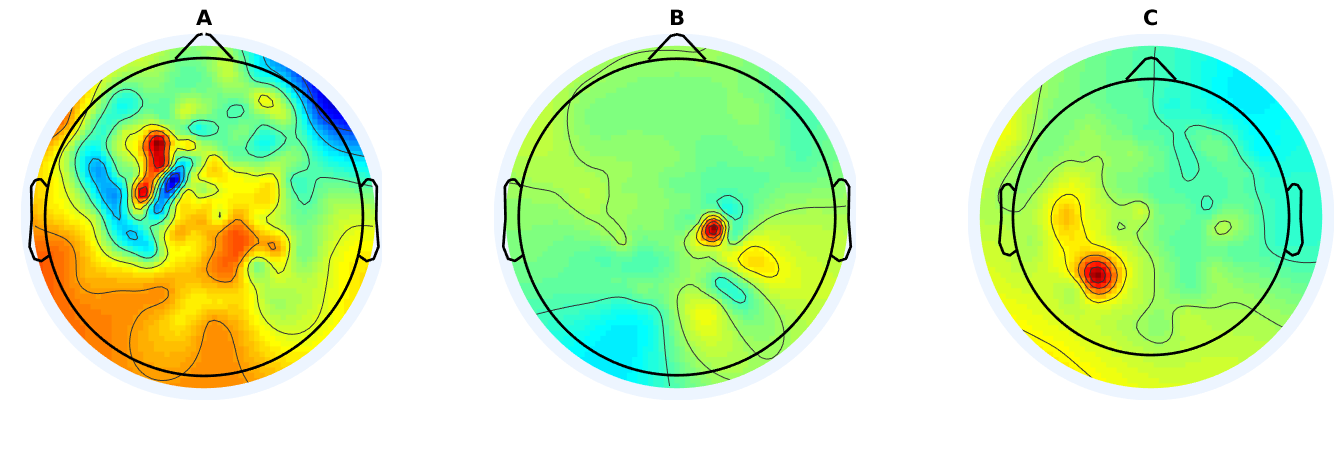
\includegraphics[width=\linewidth]{AllComponents.png}
  \caption{Graphical illustrations (using \cite{Delorme04eeglab}) of the independent components with features most correlated with audio features, from left to right, /{\em pah}/, /{\em pah tah kah}/ and verb generation experiments. These are generated using the ICA weight matrix interpolated over MEG sensor locations. }
  \label{fig:components}
\end{figure}
 
\subsubsection{All features vs. age}

When correlating with age, 172 features were found to have significant values, all of which were MEG features. This includes the autocorrelation features of eight (ICA) components -- including the first (highest entropy) component -- in addition to the entire available frequency spectrum of four of these components and one other. The fact that spectral features are relatively strongly correlated with age might provide evidence that synchronization may be a distinguishing factor across age, but additional feature analysis will be necessary to confirm this.

The correlation of a single computed component has correlation coefficients $\text{abs}(r)>0.3$ for nearly all of its features, which was true of no other components considered. Examining the physical representation of these components with respect to each of the three experiments, there were no discernible similarities to note. Three other components also had features with correlation $\text{abs}(r)>0.3$, for features that corresponded to various mean variants.

\subsection{Regression}

\begin{table}[t]
  \centering
  \label{tab:reg_results}
  \begin{tabular}{| l | c | c |}
    \toprule
    \multicolumn{1}{l}{\textbf{Feature set}} & \multicolumn{1}{c}{\textbf{Mean}} & \multicolumn{1}{c}{\textbf{Variance}} \\
    \toprule
        Audio~~~                             & ~~~$4.103$         &     $0.473$       \\
        MEG~~~                               & ~~~$4.896$         &     $0.234$       \\
        Audio+MEG~~~                         & ~~~$4.109$         &     $0.244$       \\

        \midrule
       
        MEG (red.)~~~                        & ~~~$5.081$         &     \textbf{0.142}       \\
        Audio+MEG (red.)~~~                  & ~~~\textbf{3.370}         &     $0.248$       \\

        \bottomrule
  \end{tabular}
  \caption{Root mean squared error (RMSE), in years, of 10-fold cross validation for each of the feature sets. Audio features combined with reduced MEG features show the best prediction capability. Bold indicates best performance.}
\end{table}

The regression performance across the 10 folds seems to suggest that a multilinear regression model trained using both audio and the reduced (i.e., highly correlated) MEG feature sets performs better than either Audio or MEG feature sets alone. Without  reducing the MEG feature set, regression performance is no better than that for Audio alone. Models trained using some MEG features also  perform more consistently (i.e., with lower variance) than with Audio features exclusively.

When trained using the highly correlated MEG features, regression performance is nearly equivalent to its exhaustive counterpart. There is a fairly marked reduction in variance, but performance does not increase until Audio and MEG features are combined. This may be surprising, considering that the MEG features are relatively correlated with age. This could suggest somewhat complementary information between data sets. % FR: in future, a measure of mutual information should be computed.

Table \ref{tab:reg_results} shows the means and variances of root mean squared error (RMSE) values on regression, given various combinations of feature sets. Clearly, combining audio features with a reduced set of MEG features result in the best accuracy on average. An $n$-way ANOVA confirms a significant effect of the feature type on regression accuracy ($F_{4,49} = 51.05$, $p<0.001$), with the combined Audio + reduced MEG features being significantly more accurate than {\em each} of the other combinations, according to right-tailed $t$-tests, after correcting $\alpha$, with Bonferroni, for multiple comparisons.

\subsection{Feature Based Classification}

\begin{table}[t]
  \centering
  \label{tab:feat_results}
  \begin{tabular}{l l | c | c}
    \textbf{Feature set} & Model & \textbf{Mean \%} & \textbf{Variance \%} \\
    \toprule
    \multirow{3}{*}{Audio}
    & Logistic Regression & 25.3 & 3.20  \\
    & Linear SVM          & NaN & NaN  \\
    & Shallow NN          & 44.7 & 1.33  \\
    \midrule
    \multirow{3}{*}{MEG}
    & Logistic Regression & 44.4 & 10.9  \\
    & Linear SVM          & NaN & NaN  \\
    & Shallow NN          & NaN & NaN  \\
    \midrule
    \multirow{3}{*}{Audio + MEG}
    & Logistic Regression & 14.0 & 1.14  \\
    & Linear SVM          & NaN & NaN  \\
    & Shallow NN          & 64.0 & 5.03  \\
    \bottomrule
  \end{tabular}
  \caption{Classification accuracy using one of three datasets, and three different basic classifier models.}
\end{table}

We found very little success in training the recurrent neural networks using the feature based datasets, furthermore the addition of attention made no sugnificant improvement.

% I don't think much space should be devoted to the analysis of the parameters of these models

\subsection{End-to-End Classification}

\subsubsection{Primary Dataset}

\begin{table}[t]
  \centering
  \label{tab:end2end_results}
  \begin{tabular}{l l | c | c}
    \textbf{Feature set} & Model & \textbf{Mean \%} & \textbf{Variance \%} \\
    \toprule
    \multirow{3}{*}{No Augmentation}
    & Logistic Regression & NaN & Nan  \\
    & Linear SVM          & NaN & NaN  \\
    & Shallow NN          & NaN & NaN  \\
    \midrule

    \bottomrule
  \end{tabular}
  \caption{Classification accuracy using real data input under different augmentation strategies and models.}
\end{table}

\subsubsection{Learned Features}

\subsubsection{Secondary Dataset}

\subsubsection{Learned Features}

\section{Discussion}

%% Taken from IS paper, still needs to be changed

This work is a preliminary combination and comparison of aligned Audio and MEG data, in a few speech production tasks, across children of various ages. While there exist relatively few correlations {\em across} these modalities -- and those that exist are relatively low -- they both provide similarly informative predictive power towards age regression, and even more so when combined.

To compare with the `optimal' reduced set of features, according to absolute correlation {\em and} their $p$-values, we also {\em randomly} extract a subset of 172 features. Performing multilinear regression on this random selection of features remains insignificantly different than using all features. Finally, we also considered a set of the 172 most correlated MEG features {\em among those} with $p \geq 0.0001$, which accounts for high, but potentially quite variable, correlations. Surprisingly, this improved accuracy slightly on average over using all features, but with a much larger variance (i.e., $\geq 0.9$). The optimum solution remains to force $p<0.0001$ for each correlation. These {\em ad hoc} analyses seem to suggest that increases in performance depend not on merely reducing dimensionality blindly, but on selecting {\em consistently} correlating features.

Performing ICA separately for each stimulus results in different components, naturally. In other words, component $c_i$ with respect to the /{\em pah}/ data is different than component $c_i'$ with respect to the VG data. Future work should consider the sensitivity of any analysis to the stimulus, and be able to generalize ICA analyses that were performed on slightly different data sets.

Audio frequencies just below 400 Hz often correlate with MEG features. For the /{\em pah}/ and /{\em pah tah kah}/ stimuli, our initial hypothesis was that these would relate to F0, or the formant structure of the phone /{\em ah}/. However, whether this is the case remains to be determined.

This paper provides a strong baseline indicating that MEG data can provide a significant improvement to age detection, over Audio features alone. We are currently considering more complex models that relate MEG and audio features in conjunction with other features. Although this dataset is relatively large, considering the population and equipment, it will be important to evaluate whether it is sufficiently large to train modern regularized methods in deep learning.

%% New Discussion points - All out of order, need to be organized and extended

What is important to note, is that although some models do succeed in classifying the examples in the primary dataset, many models fail to perform better than random chance. This implies that the architecture selected is of critical importance, and in many cases will not suffice to try incompatible architectures for {\em good enough} classification performance. We see this as further indication that the application of deep-learning here is appropriate and necessitates continued development to establish a tool-set of appropriate architectures and stronger guiding principles for this type of data.

What might be interesting to note, given the relatively little data in comparison with larger datasets used in applications like image and language processing, is the lack of early overfitting. Typically with a limited amount of data and such expressive models as were tested, overfitting is a primary concern. This was mostly the case when using the BCI IV 2a dataset, but much less so with the MEG dataset which, when using the entire training set, at times struggled to perform better than chance unless without the use of one of the more successful architectures.

We spent some time exploring CNN architectures that developed features using data across time and space, but found very little success with these methods, (these experiments were very preliminary and consisted of a few heuristic selections of parameters). Typically the failure was not the result of over-fitting

{\em Might spend some more time experimenting with the following observation:} When experimenting with crop strategies using the supplementary dataset in particular, it seemed apparent that taking crops from significantly before the onset of the experiment event the model became difficult to train. This may have been noticeable here because the recording are quite long (relative to the primary dataset). This may at first glance somewhat obvious, but it further suggests that the model genuinely is learning to distinguish input due to the event itself, rather than some other distinctiveness that may separate the trials, and thus it is a good sanity check.

\begin{itemize}
\item future work: seq2seq model that predicts phonemes/connects to some other pre-canned speech generation
\item future work: Consider that inter-channel correlations tended to be significant, devise back-prop trainable functions that use this? Or is this idea a bit too nebulous?
\end{itemize}


%% Discussion points that may be better suited to an appendix, but I wanted to save them as they came up.

We are inclined to believe that despite their power in end-to-end learning, convolutional networks may not perform well with engineered features in this context because few generalizable combinations could be found. It is conceivable that with the selected features it is difficult for the network to develop higher level abstractions. Following this line of reasoning, the SVMs could therefore have been powerful as a result of this, as most neural network based classifiers should be developing some sort of abstraction and the SVMs are mostly finding an ideal way to separate this data. That being said, employing attention to the SVMs should have performed no worse than SVMs with attention. The attention mechanism should have aided in remedying the downside of flattening the data when using classifiers that expect input vectors, but are time-series data. However this may be due to some hitherto unknown difficulty in training attention mechanisms with L2-SVM output layers.

During the initial evaluation of each model, we considered L2 SVM output layers as described in \cite{l2svmuoftpaper}, but found that they performed no better than a softmax output layer and tended if anything to perform slightly worse overall.

Towards determining if the PA/PDK vocalization trials or the verb generation experiment trials had a greater impact on performance in the end-to-end learning, we trained both the 2D projected attention, and convolutional attention models using each of these datasets seperately. Interestingly they seemed to have difficulty outperforming random chance on their own (details not reported), suggesting that despite being slightly different experiments an increase in datapoints is crucial to enabling the performance of these more powerful ML models.

\section{Acknowledgements}

We thank Rui Janson for his help performing automated EOG removal.

\appendix{Hyper-parameter Search}

All hyper-parameter searches were done using hyperopt \cite{Bergstra2013}
%% Describe spaces used for search

\bibliographystyle{frontiersinSCNS_ENG_HUMS} % for Science, Engineering and Humanities and Social Sciences articles, for Humanities and Social Sciences articles please include page numbers in the in-text citations
%\bibliographystyle{frontiersinHLTH&FPHY} % for Health, Physics and Mathematics articles
\bibliography{frontiers}

\end{document}
